%
\begin{isabellebody}%
\def\isabellecontext{Presentation}%
%
\isadelimtheory
%
\endisadelimtheory
%
\isatagtheory
\isacommand{theory}\isamarkupfalse%
\ Presentation\isanewline
\isakeyword{imports}\ Pure\isanewline
\isakeyword{begin}%
\endisatagtheory
{\isafoldtheory}%
%
\isadelimtheory
%
\endisadelimtheory
%
\isamarkupchapter{Presenting theories \label{ch:present}%
}
\isamarkuptrue%
%
\begin{isamarkuptext}%
Isabelle provides several ways to present the outcome of formal
  developments, including WWW-based browsable libraries or actual
  printable documents.  Presentation is centered around the concept of
  \emph{logic sessions}.  The global session structure is that of a
  tree, with Isabelle Pure at its root, further object-logics derived
  (e.g.\ HOLCF from HOL, and HOL from Pure), and application sessions
  in leaf positions (usually without a separate image).

  The Isabelle tools \indexref{}{tool}{mkdir}\hyperlink{tool.mkdir}{\mbox{\isa{\isatt{mkdir}}}} and \indexref{}{tool}{make}\hyperlink{tool.make}{\mbox{\isa{\isatt{make}}}} provide
  the primary means for managing Isabelle sessions, including proper
  setup for presentation.  Here the \indexref{}{tool}{usedir}\hyperlink{tool.usedir}{\mbox{\isa{\isatt{usedir}}}} tool takes care
  to let \indexref{}{executable}{isabelle-process}\hyperlink{executable.isabelle-process}{\mbox{\isa{\isatt{isabelle{\isacharminus}process}}}} process run any
  additional stages required for document preparation, notably the
  tools \indexref{}{tool}{document}\hyperlink{tool.document}{\mbox{\isa{\isatt{document}}}} and \indexref{}{tool}{latex}\hyperlink{tool.latex}{\mbox{\isa{\isatt{latex}}}}.  The complete tool
  chain for managing batch-mode Isabelle sessions is illustrated in
  \figref{fig:session-tools}.

  \begin{figure}[htbp]
  \begin{center}
  \begin{tabular}{lp{0.6\textwidth}}

      \verb|isabelle| \indexref{}{tool}{mkdir}\hyperlink{tool.mkdir}{\mbox{\isa{\isatt{mkdir}}}} & invoked once by the user
      to create the initial source setup (common \verb|IsaMakefile| plus a single session directory); \\

      \verb|isabelle| \hyperlink{tool.make}{\mbox{\isa{\isatt{make}}}} & invoked repeatedly by the
      user to keep session output up-to-date (HTML, documents etc.); \\

      \verb|isabelle| \hyperlink{tool.usedir}{\mbox{\isa{\isatt{usedir}}}} & part of the standard
      \verb|IsaMakefile| entry of a session; \\

      \hyperlink{executable.isabelle-process}{\mbox{\isa{\isatt{isabelle{\isacharminus}process}}}} & run through \verb|isabelle| \indexref{}{tool}{usedir}\hyperlink{tool.usedir}{\mbox{\isa{\isatt{usedir}}}}; \\

      \verb|isabelle| \indexref{}{tool}{document}\hyperlink{tool.document}{\mbox{\isa{\isatt{document}}}} & run by the Isabelle
      process if document preparation is enabled; \\

      \verb|isabelle| \indexref{}{tool}{latex}\hyperlink{tool.latex}{\mbox{\isa{\isatt{latex}}}} & universal {\LaTeX} tool
      wrapper invoked multiple times by \verb|isabelle| \indexref{}{tool}{document}\hyperlink{tool.document}{\mbox{\isa{\isatt{document}}}}; also useful for manual experiments; \\

  \end{tabular}
  \caption{The tool chain of Isabelle session presentation} \label{fig:session-tools}
  \end{center}
  \end{figure}%
\end{isamarkuptext}%
\isamarkuptrue%
%
\isamarkupsection{Generating theory browser information \label{sec:info}%
}
\isamarkuptrue%
%
\begin{isamarkuptext}%
\index{theory browsing information|bold}

  As a side-effect of running a logic sessions, Isabelle is able to
  generate theory browsing information, including HTML documents that
  show a theory's definition, the theorems proved in its ML file and
  the relationship with its ancestors and descendants.  Besides the
  HTML file that is generated for every theory, Isabelle stores links
  to all theories in an index file. These indexes are linked with
  other indexes to represent the overall tree structure of logic
  sessions.

  Isabelle also generates graph files that represent the theory
  hierarchy of a logic.  There is a graph browser Java applet embedded
  in the generated HTML pages, and also a stand-alone application that
  allows browsing theory graphs without having to start a WWW client
  first.  The latter version also includes features such as generating
  Postscript files, which are not available in the applet version.
  See \secref{sec:browse} for further information.

  \medskip

  The easiest way to let Isabelle generate theory browsing information
  for existing sessions is to append ``\verb|-i true|'' to the
  \indexref{}{setting}{ISABELLE\_USEDIR\_OPTIONS}\hyperlink{setting.ISABELLE-USEDIR-OPTIONS}{\mbox{\isa{\isatt{ISABELLE{\isacharunderscore}USEDIR{\isacharunderscore}OPTIONS}}}} before invoking \verb|isabelle| \hyperlink{tool.make}{\mbox{\isa{\isatt{make}}}} (or \hyperlink{file.$ISABELLE-HOME/build}{\mbox{\isa{\isatt{{\isachardollar}ISABELLE{\isacharunderscore}HOME{\isacharslash}build}}}}).  For
  example, add something like this to your Isabelle settings file

\begin{ttbox}
ISABELLE_USEDIR_OPTIONS="-i true"
\end{ttbox}

  and then change into the \hyperlink{file.~~/src/FOL}{\mbox{\isa{\isatt{{\isachartilde}{\isachartilde}{\isacharslash}src{\isacharslash}FOL}}}} directory and run
  \verb|isabelle| \hyperlink{tool.make}{\mbox{\isa{\isatt{make}}}}, or even \verb|isabelle| \hyperlink{tool.make}{\mbox{\isa{\isatt{make}}}}~\verb|all|.  The presentation output will appear in
  \verb|ISABELLE_BROWSER_INFO/FOL|, which usually refers to
  \verb|~/.isabelle/browser_info/FOL|.  Note that option
  \verb|-v true| will make the internal runs of \hyperlink{tool.usedir}{\mbox{\isa{\isatt{usedir}}}}
  more explicit about such details.

  Many standard Isabelle sessions (such as \hyperlink{file.~~/src/HOL/ex}{\mbox{\isa{\isatt{{\isachartilde}{\isachartilde}{\isacharslash}src{\isacharslash}HOL{\isacharslash}ex}}}})
  also provide actual printable documents.  These are prepared
  automatically as well if enabled like this, using the \verb|-d| option
\begin{ttbox}
ISABELLE_USEDIR_OPTIONS="-i true -d dvi"
\end{ttbox}
  Enabling options \verb|-i| and \verb|-d|
  simultaneously as shown above causes an appropriate ``document''
  link to be included in the HTML index.  Documents (or raw document
  sources) may be generated independently of browser information as
  well, see \secref{sec:tool-document} for further details.

  \bigskip The theory browsing information is stored in a
  sub-directory directory determined by the \indexref{}{setting}{ISABELLE\_BROWSER\_INFO}\hyperlink{setting.ISABELLE-BROWSER-INFO}{\mbox{\isa{\isatt{ISABELLE{\isacharunderscore}BROWSER{\isacharunderscore}INFO}}}} setting plus a prefix corresponding to the
  session identifier (according to the tree structure of sub-sessions
  by default).  A complete WWW view of all standard object-logics and
  examples of the Isabelle distribution is available at the usual
  Isabelle sites:
  \begin{center}\small
  \begin{tabular}{l}
    \url{http://isabelle.in.tum.de/dist/library/} \\
    \url{http://www.cl.cam.ac.uk/research/hvg/Isabelle/dist/library/} \\
    \url{http://mirror.cse.unsw.edu.au/pub/isabelle/dist/library/} \\
  \end{tabular}
  \end{center}
  
  \medskip In order to present your own theories on the web, simply
  copy the corresponding subdirectory from \hyperlink{setting.ISABELLE-BROWSER-INFO}{\mbox{\isa{\isatt{ISABELLE{\isacharunderscore}BROWSER{\isacharunderscore}INFO}}}} to your WWW server, having generated browser
  info like this:
\begin{ttbox}
isabelle usedir -i true HOL Foo
\end{ttbox}

  This assumes that directory \verb|Foo| contains some \verb|ROOT.ML| file to load all your theories, and HOL is your parent
  logic image (\verb|isabelle| \indexref{}{tool}{mkdir}\hyperlink{tool.mkdir}{\mbox{\isa{\isatt{mkdir}}}} assists in
  setting up Isabelle session directories.  Theory browser information
  for HOL should have been generated already beforehand.
  Alternatively, one may specify an external link to an existing body
  of HTML data by giving \hyperlink{tool.usedir}{\mbox{\isa{\isatt{usedir}}}} a \verb|-P| option like
  this:
\begin{ttbox}
isabelle usedir -i true -P http://isabelle.in.tum.de/library/ HOL Foo
\end{ttbox}

  \medskip For production use, the \hyperlink{tool.usedir}{\mbox{\isa{\isatt{usedir}}}} tool is usually
  invoked in an appropriate \verb|IsaMakefile|, via the Isabelle
  \hyperlink{tool.make}{\mbox{\isa{\isatt{make}}}} tool.  There is a separate \hyperlink{tool.mkdir}{\mbox{\isa{\isatt{mkdir}}}} tool to
  provide easy setup of all this, with only minimal manual editing
  required.
\begin{ttbox}
isabelle mkdir HOL Foo && isabelle make
\end{ttbox}
  See \secref{sec:tool-mkdir} for more information on preparing
  Isabelle session directories, including the setup for documents.%
\end{isamarkuptext}%
\isamarkuptrue%
%
\isamarkupsection{Browsing theory graphs \label{sec:browse}%
}
\isamarkuptrue%
%
\begin{isamarkuptext}%
\index{theory graph browser|bold} 

  The Isabelle graph browser is a general tool for visualizing
  dependency graphs.  Certain nodes of the graph (i.e.~theories) can
  be grouped together in ``directories'', whose contents may be
  hidden, thus enabling the user to collapse irrelevant portions of
  information.  The browser is written in Java, it can be used both as
  a stand-alone application and as an applet.  Note that the option
  \verb|-g| of \verb|isabelle| \indexref{}{tool}{usedir}\hyperlink{tool.usedir}{\mbox{\isa{\isatt{usedir}}}} creates
  graph presentations in batch mode for inclusion in session
  documents.%
\end{isamarkuptext}%
\isamarkuptrue%
%
\isamarkupsubsection{Invoking the graph browser%
}
\isamarkuptrue%
%
\begin{isamarkuptext}%
The stand-alone version of the graph browser is wrapped up as an
  Isabelle tool called \indexdef{}{tool}{browser}\hypertarget{tool.browser}{\hyperlink{tool.browser}{\mbox{\isa{\isatt{browser}}}}}:

\begin{ttbox}
Usage: browser [OPTIONS] [GRAPHFILE]

  Options are:
    -b           Admin/build only
    -c           cleanup -- remove GRAPHFILE after use
    -o FILE      output to FILE (ps, eps, pdf)
\end{ttbox}
  When no filename is specified, the browser automatically changes to
  the directory \hyperlink{setting.ISABELLE-BROWSER-INFO}{\mbox{\isa{\isatt{ISABELLE{\isacharunderscore}BROWSER{\isacharunderscore}INFO}}}}.

  \medskip The \verb|-b| option indicates that this is for
  administrative build only, i.e.\ no browser popup if no files are
  given.

  The \verb|-c| option causes the input file to be removed
  after use.

  The \verb|-o| option indicates batch-mode operation, with the
  output written to the indicated file; note that \verb|pdf|
  produces an \verb|eps| copy as well.

  \medskip The applet version of the browser is part of the standard
  WWW theory presentation, see the link ``theory dependencies'' within
  each session index.%
\end{isamarkuptext}%
\isamarkuptrue%
%
\isamarkupsubsection{Using the graph browser%
}
\isamarkuptrue%
%
\begin{isamarkuptext}%
The browser's main window, which is shown in
  \figref{fig:browserwindow}, consists of two sub-windows.  In the
  left sub-window, the directory tree is displayed. The graph itself
  is displayed in the right sub-window.

  \begin{figure}[ht]
  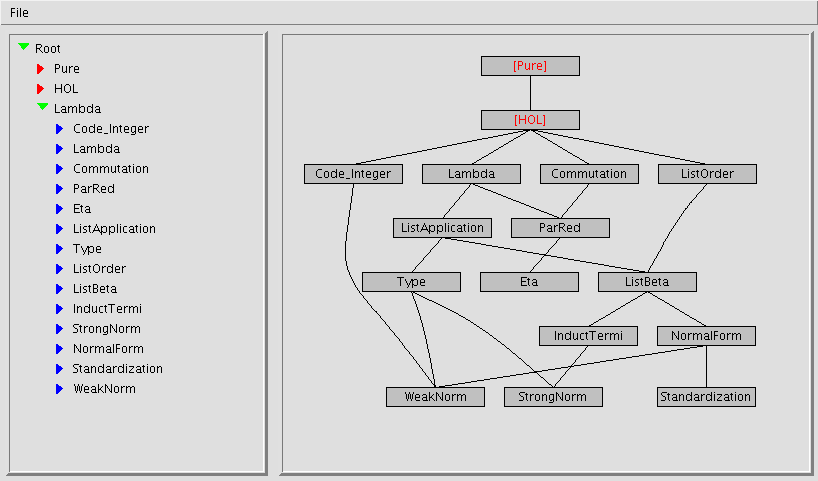
\includegraphics[width=\textwidth]{browser_screenshot}
  \caption{\label{fig:browserwindow} Browser main window}
  \end{figure}%
\end{isamarkuptext}%
\isamarkuptrue%
%
\isamarkupsubsubsection{The directory tree window%
}
\isamarkuptrue%
%
\begin{isamarkuptext}%
We describe the usage of the directory browser and the meaning of
  the different items in the browser window.

  \begin{itemize}
  
  \item A red arrow before a directory name indicates that the
  directory is currently ``folded'', i.e.~the nodes in this directory
  are collapsed to one single node. In the right sub-window, the names
  of nodes corresponding to folded directories are enclosed in square
  brackets and displayed in red color.
  
  \item A green downward arrow before a directory name indicates that
  the directory is currently ``unfolded''. It can be folded by
  clicking on the directory name.  Clicking on the name for a second
  time unfolds the directory again.  Alternatively, a directory can
  also be unfolded by clicking on the corresponding node in the right
  sub-window.
  
  \item Blue arrows stand before ordinary node names. When clicking on
  such a name (i.e.\ that of a theory), the graph display window
  focuses to the corresponding node. Double clicking invokes a text
  viewer window in which the contents of the theory file are
  displayed.

  \end{itemize}%
\end{isamarkuptext}%
\isamarkuptrue%
%
\isamarkupsubsubsection{The graph display window%
}
\isamarkuptrue%
%
\begin{isamarkuptext}%
When pointing on an ordinary node, an upward and a downward arrow is
  shown.  Initially, both of these arrows are green. Clicking on the
  upward or downward arrow collapses all predecessor or successor
  nodes, respectively. The arrow's color then changes to red,
  indicating that the predecessor or successor nodes are currently
  collapsed. The node corresponding to the collapsed nodes has the
  name ``\verb|[....]|''. To uncollapse the nodes again, simply
  click on the red arrow or on the node with the name ``\verb|[....]|''. Similar to the directory browser, the contents of
  theory files can be displayed by double clicking on the
  corresponding node.%
\end{isamarkuptext}%
\isamarkuptrue%
%
\isamarkupsubsubsection{The ``File'' menu%
}
\isamarkuptrue%
%
\begin{isamarkuptext}%
Due to Java Applet security restrictions this menu is only available
  in the full application version. The meaning of the menu items is as
  follows:

  \begin{description}
  
  \item[Open \dots] Open a new graph file.
  
  \item[Export to PostScript] Outputs the current graph in Postscript
  format, appropriately scaled to fit on one single sheet of A4 paper.
  The resulting file can be printed directly.
  
  \item[Export to EPS] Outputs the current graph in Encapsulated
  Postscript format. The resulting file can be included in other
  documents.

  \item[Quit] Quit the graph browser.

  \end{description}%
\end{isamarkuptext}%
\isamarkuptrue%
%
\isamarkupsubsection{Syntax of graph definition files%
}
\isamarkuptrue%
%
\begin{isamarkuptext}%
A graph definition file has the following syntax:

  \begin{center}\small
  \begin{tabular}{rcl}
    \isa{graph} & \isa{{\isachardoublequote}{\isacharequal}{\isachardoublequote}} & \isa{{\isachardoublequote}{\isacharbraceleft}\ vertex{\isachardoublequote}}~\verb|;|~\isa{{\isachardoublequote}{\isacharbraceright}{\isacharplus}{\isachardoublequote}} \\
    \isa{vertex} & \isa{{\isachardoublequote}{\isacharequal}{\isachardoublequote}} & \isa{{\isachardoublequote}vertex{\isacharunderscore}name\ vertex{\isacharunderscore}ID\ dir{\isacharunderscore}name\ {\isacharbrackleft}{\isachardoublequote}}~\verb|+|~\isa{{\isachardoublequote}{\isacharbrackright}\ path\ {\isacharbrackleft}{\isachardoublequote}}~\verb|<|~\isa{{\isachardoublequote}{\isacharbar}{\isachardoublequote}}~\verb|>|~\isa{{\isachardoublequote}{\isacharbrackright}\ {\isacharbraceleft}\ vertex{\isacharunderscore}ID\ {\isacharbraceright}{\isacharasterisk}{\isachardoublequote}}
  \end{tabular}
  \end{center}

  The meaning of the items in a vertex description is as follows:

  \begin{description}
  
  \item[\isa{vertex{\isacharunderscore}name}] The name of the vertex.
  
  \item[\isa{vertex{\isacharunderscore}ID}] The vertex identifier. Note that there may
  be several vertices with equal names, whereas identifiers must be
  unique.
  
  \item[\isa{dir{\isacharunderscore}name}] The name of the ``directory'' the vertex
  should be placed in.  A ``\verb|+|'' sign after \isa{dir{\isacharunderscore}name} indicates that the nodes in the directory are initially
  visible. Directories are initially invisible by default.
  
  \item[\isa{path}] The path of the corresponding theory file. This
  is specified relatively to the path of the graph definition file.
  
  \item[List of successor/predecessor nodes] A ``\verb|<|''
  sign before the list means that successor nodes are listed, a
  ``\verb|>|'' sign means that predecessor nodes are listed. If
  neither ``\verb|<|'' nor ``\verb|>|'' is found, the
  browser assumes that successor nodes are listed.

  \end{description}%
\end{isamarkuptext}%
\isamarkuptrue%
%
\isamarkupsection{Creating Isabelle session directories
  \label{sec:tool-mkdir}%
}
\isamarkuptrue%
%
\begin{isamarkuptext}%
The \indexdef{}{tool}{mkdir}\hypertarget{tool.mkdir}{\hyperlink{tool.mkdir}{\mbox{\isa{\isatt{mkdir}}}}} utility prepares Isabelle session source
  directories, including a sensible default setup of \verb|IsaMakefile|, \verb|ROOT.ML|, and a \verb|document|
  directory with a minimal \verb|root.tex| that is sufficient to
  print all theories of the session (in the order of appearance); see
  \secref{sec:tool-document} for further information on Isabelle
  document preparation.  The usage of \verb|isabelle| \hyperlink{tool.mkdir}{\mbox{\isa{\isatt{mkdir}}}} is:

\begin{ttbox}
Usage: mkdir [OPTIONS] [LOGIC] NAME

  Options are:
    -I FILE      alternative IsaMakefile output
    -P           include parent logic target
    -b           setup build mode (session outputs heap image)
    -q           quiet mode

  Prepare session directory, including IsaMakefile and document source,
  with parent LOGIC (default ISABELLE_LOGIC=\$ISABELLE_LOGIC)
\end{ttbox}

  The \hyperlink{tool.mkdir}{\mbox{\isa{\isatt{mkdir}}}} tool is conservative in the sense that any
  existing \verb|IsaMakefile| etc.\ is left unchanged.  Thus it
  is safe to invoke it multiple times, although later runs may not
  have the desired effect.

  Note that \hyperlink{tool.mkdir}{\mbox{\isa{\isatt{mkdir}}}} is unable to change \verb|IsaMakefile|
  incrementally --- manual changes are required for multiple
  sub-sessions.  On order to get an initial working session, the only
  editing needed is to add appropriate \verb|use_thy| calls to the
  generated \verb|ROOT.ML| file.%
\end{isamarkuptext}%
\isamarkuptrue%
%
\isamarkupsubsubsection{Options%
}
\isamarkuptrue%
%
\begin{isamarkuptext}%
The \verb|-I| option specifies an alternative to \verb|IsaMakefile| for dependencies.  Note that ``\verb|-|'' refers
  to \emph{stdout}, i.e.\ ``\verb|-I-|'' provides an easy way
  to peek at \hyperlink{tool.mkdir}{\mbox{\isa{\isatt{mkdir}}}}'s idea of \hyperlink{tool.make}{\mbox{\isa{\isatt{make}}}} setup required for
  some particular of Isabelle session.

  \medskip The \verb|-P| option includes a target for the
  parent \verb|LOGIC| session in the generated \verb|IsaMakefile|.  The corresponding sources are assumed to be located
  within the Isabelle distribution.

  \medskip The \verb|-b| option sets up the current directory
  as the base for a new session that provides an actual logic image,
  as opposed to one that only runs several theories based on an
  existing image.  Note that in the latter case, everything except
  \verb|IsaMakefile| would be placed into a separate directory
  \verb|NAME|, rather than the current one.  See
  \secref{sec:tool-usedir} for further information on \emph{build
  mode} vs.\ \emph{example mode} of the \hyperlink{tool.usedir}{\mbox{\isa{\isatt{usedir}}}} utility.

  \medskip The \verb|-q| option enables quiet mode, suppressing
  further notes on how to proceed.%
\end{isamarkuptext}%
\isamarkuptrue%
%
\isamarkupsubsubsection{Examples%
}
\isamarkuptrue%
%
\begin{isamarkuptext}%
The standard setup of a single ``example session'' based on the
  default logic, with proper document generation is generated like
  this:
\begin{ttbox}
isabelle mkdir Foo && isabelle make
\end{ttbox}

  \noindent The theory sources should be put into the \verb|Foo|
  directory, and its \verb|ROOT.ML| should be edited to load all
  required theories.  Invoking \verb|isabelle| \hyperlink{tool.make}{\mbox{\isa{\isatt{make}}}} again
  would run the whole session, generating browser information and the
  document automatically.  The \verb|IsaMakefile| is typically
  tuned manually later, e.g.\ adding source dependencies, or changing
  the options passed to \hyperlink{tool.usedir}{\mbox{\isa{\isatt{usedir}}}}.

  \medskip Large projects may demand further sessions, potentially
  with separate logic images being created.  This usually requires
  manual editing of the generated \verb|IsaMakefile|, which is
  meant to cover all of the sub-session directories at the same time
  (this is the deeper reasong why \verb|IsaMakefile| is not made
  part of the initial session directory created by \verb|isabelle| \hyperlink{tool.mkdir}{\mbox{\isa{\isatt{mkdir}}}}).  See \hyperlink{file.~~/src/HOL/IsaMakefile}{\mbox{\isa{\isatt{{\isachartilde}{\isachartilde}{\isacharslash}src{\isacharslash}HOL{\isacharslash}IsaMakefile}}}} for
  a full-blown example.%
\end{isamarkuptext}%
\isamarkuptrue%
%
\isamarkupsection{Running Isabelle sessions \label{sec:tool-usedir}%
}
\isamarkuptrue%
%
\begin{isamarkuptext}%
The \indexdef{}{tool}{usedir}\hypertarget{tool.usedir}{\hyperlink{tool.usedir}{\mbox{\isa{\isatt{usedir}}}}} utility builds object-logic images, or runs
  example sessions based on existing logics. Its usage is:
\begin{ttbox}

Usage: usedir [OPTIONS] LOGIC NAME

  Options are:
    -C BOOL      copy existing document directory to -D PATH (default true)
    -D PATH      dump generated document sources into PATH
    -M MAX       multithreading: maximum number of worker threads (default 1)
    -P PATH      set path for remote theory browsing information
    -T LEVEL     multithreading: trace level (default 0)
    -V VERSION   declare alternative document VERSION
    -b           build mode (output heap image, using current dir)
    -d FORMAT    build document as FORMAT (default false)
    -f NAME      use ML file NAME (default ROOT.ML)
    -g BOOL      generate session graph image for document (default false)
    -i BOOL      generate theory browser information (default false)
    -m MODE      add print mode for output
    -p LEVEL     set level of detail for proof objects (default 0)
    -q LEVEL     set level of parallel proof checking (default 1)
    -r           reset session path
    -s NAME      override session NAME
    -t BOOL      internal session timing (default false)
    -v BOOL      be verbose (default false)

  Build object-logic or run examples. Also creates browsing
  information (HTML etc.) according to settings.

  ISABELLE_USEDIR_OPTIONS=

  ML_PLATFORM=x86-linux
  ML_HOME=/usr/local/polyml-5.2.1/x86-linux
  ML_SYSTEM=polyml-5.2.1
  ML_OPTIONS=-H 500
\end{ttbox}

  Note that the value of the \indexref{}{setting}{ISABELLE\_USEDIR\_OPTIONS}\hyperlink{setting.ISABELLE-USEDIR-OPTIONS}{\mbox{\isa{\isatt{ISABELLE{\isacharunderscore}USEDIR{\isacharunderscore}OPTIONS}}}}
  setting is implicitly prefixed to \emph{any} \hyperlink{tool.usedir}{\mbox{\isa{\isatt{usedir}}}}
  call. Since the \verb|IsaMakefile|s of all object-logics
  distributed with Isabelle just invoke \hyperlink{tool.usedir}{\mbox{\isa{\isatt{usedir}}}} for the real
  work, one may control compilation options globally via above
  variable. In particular, generation of \rmindex{HTML} browsing
  information and document preparation is controlled here.%
\end{isamarkuptext}%
\isamarkuptrue%
%
\isamarkupsubsubsection{Options%
}
\isamarkuptrue%
%
\begin{isamarkuptext}%
Basically, there are two different modes of operation: \emph{build
  mode} (enabled through the \verb|-b| option) and
  \emph{example mode} (default).

  Calling \hyperlink{tool.usedir}{\mbox{\isa{\isatt{usedir}}}} with \verb|-b| runs \hyperlink{executable.isabelle-process}{\mbox{\isa{\isatt{isabelle{\isacharminus}process}}}} with input image \verb|LOGIC| and output to
  \verb|NAME|, as provided on the command line. This will be a
  batch session, running \verb|ROOT.ML| from the current
  directory and then quitting.  It is assumed that \verb|ROOT.ML|
  contains all ML commands required to build the logic.

  In example mode, \hyperlink{tool.usedir}{\mbox{\isa{\isatt{usedir}}}} runs a read-only session of
  \verb|LOGIC| and automatically runs \verb|ROOT.ML| from
  within directory \verb|NAME|.  It assumes that this file
  contains appropriate ML commands to run the desired examples.

  \medskip The \verb|-i| option controls theory browser data
  generation. It may be explicitly turned on or off --- as usual, the
  last occurrence of \verb|-i| on the command line wins.

  The \verb|-P| option specifies a path (or actual URL) to be
  prefixed to any \emph{non-local} reference of existing theories.
  Thus user sessions may easily link to existing Isabelle libraries
  already present on the WWW.

  The \verb|-m| options specifies additional print modes to be
  activated temporarily while the session is processed.

  \medskip The \verb|-d| option controls document preparation.
  Valid arguments are \verb|false| (do not prepare any document;
  this is default), or any of \verb|dvi|, \verb|dvi.gz|,
  \verb|ps|, \verb|ps.gz|, \verb|pdf|.  The logic
  session has to provide a properly setup \verb|document|
  directory.  See \secref{sec:tool-document} and
  \secref{sec:tool-latex} for more details.

  \medskip The \verb|-V| option declares alternative document
  versions, consisting of name/tags pairs (cf.\ options \verb|-n| and \verb|-t| of the \indexref{}{tool}{document}\hyperlink{tool.document}{\mbox{\isa{\isatt{document}}}} tool).  The
  standard document is equivalent to ``\verb|document=theory,proof,ML|'', which means that all theory begin/end
  commands, proof body texts, and ML code will be presented
  faithfully.  An alternative version ``\verb|outline=/proof/ML|'' would fold proof and ML parts, replacing the
  original text by a short place-holder.  The form ``\isa{name}\verb|=-|,'' means to remove document \isa{name} from
  the list of versions to be processed.  Any number of \verb|-V| options may be given; later declarations have precedence over
  earlier ones.

  \medskip The \verb|-g| option produces images of the theory
  dependency graph (cf.\ \secref{sec:browse}) for inclusion in the
  generated document, both as \verb|session_graph.eps| and
  \verb|session_graph.pdf| at the same time.  To include this in
  the final {\LaTeX} document one could say \verb|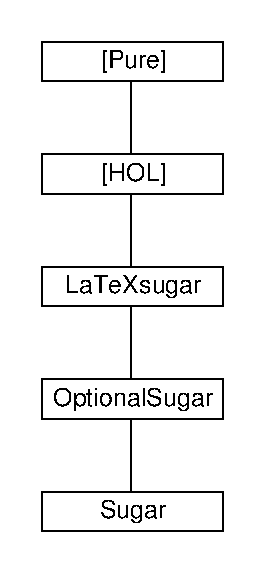
\includegraphics{session_graph}| in \verb|document/root.tex| (omitting the file-name extension enables
  {\LaTeX} to select to correct version, either for the DVI or PDF
  output path).

  \medskip The \verb|-D| option causes the generated document
  sources to be dumped at location \verb|PATH|; this path is
  relative to the session's main directory.  If the \verb|-C|
  option is true, this will include a copy of an existing \verb|document| directory as provided by the user.  For example,
  \verb|isabelle| \hyperlink{tool.usedir}{\mbox{\isa{\isatt{usedir}}}}~\verb|-D generated HOL|\isasep\isanewline%
\verb|  Foo| produces a complete set of document sources at \verb|Foo/generated|.  Subsequent invocation of \verb|isabelle| \hyperlink{tool.document}{\mbox{\isa{\isatt{document}}}}~\verb|Foo/generated| (see also
  \secref{sec:tool-document}) will process the final result
  independently of an Isabelle job.  This decoupled mode of operation
  facilitates debugging of serious {\LaTeX} errors, for example.

  \medskip The \verb|-p| option determines the level of detail
  for internal proof objects, see also the \emph{Isabelle Reference
  Manual}~\cite{isabelle-ref}.

  \medskip The \verb|-q| option specifies the level of parallel
  proof checking: \verb|0| no proofs, \verb|1| toplevel
  proofs (default), \verb|2| toplevel and nested Isar proofs.
  The resulting speedup may vary, depending on the number of worker
  threads, granularity of proofs, and whether proof terms are enabled.

  \medskip The \verb|-t| option produces a more detailed
  internal timing report of the session.

  \medskip The \verb|-v| option causes additional information
  to be printed while running the session, notably the location of
  prepared documents.

  \medskip The \verb|-M| option specifies the maximum number of
  parallel threads used for processing independent tasks when checking
  theory sources (multithreading only works on suitable ML platforms).
  The special value of \verb|0| or \verb|max| refers to the
  number of actual CPU cores of the underlying machine, which is a
  good starting point for optimal performance tuning.  The \verb|-T| option determines the level of detail in tracing output
  concerning the internal locking and scheduling in multithreaded
  operation.  This may be helpful in isolating performance
  bottle-necks, e.g.\ due to excessive wait states when locking
  critical code sections.

  \medskip Any \hyperlink{tool.usedir}{\mbox{\isa{\isatt{usedir}}}} session is named by some \emph{session
  identifier}. These accumulate, documenting the way sessions depend
  on others. For example, consider \verb|Pure/FOL/ex|, which
  refers to the examples of FOL, which in turn is built upon Pure.

  The current session's identifier is by default just the base name of
  the \verb|LOGIC| argument (in build mode), or of the \verb|NAME| argument (in example mode). This may be overridden explicitly
  via the \verb|-s| option.%
\end{isamarkuptext}%
\isamarkuptrue%
%
\isamarkupsubsubsection{Examples%
}
\isamarkuptrue%
%
\begin{isamarkuptext}%
Refer to the \verb|IsaMakefile|s of the Isabelle distribution's
  object-logics as a model for your own developments.  For example,
  see \hyperlink{file.~~/src/FOL/IsaMakefile}{\mbox{\isa{\isatt{{\isachartilde}{\isachartilde}{\isacharslash}src{\isacharslash}FOL{\isacharslash}IsaMakefile}}}}.  The Isabelle \indexref{}{tool}{mkdir}\hyperlink{tool.mkdir}{\mbox{\isa{\isatt{mkdir}}}} tool creates \verb|IsaMakefile|s with proper invocation
  of \hyperlink{tool.usedir}{\mbox{\isa{\isatt{usedir}}}} as well.%
\end{isamarkuptext}%
\isamarkuptrue%
%
\isamarkupsection{Preparing Isabelle session documents
  \label{sec:tool-document}%
}
\isamarkuptrue%
%
\begin{isamarkuptext}%
The \indexdef{}{tool}{document}\hypertarget{tool.document}{\hyperlink{tool.document}{\mbox{\isa{\isatt{document}}}}} utility prepares logic session documents,
  processing the sources both as provided by the user and generated by
  Isabelle.  Its usage is:
\begin{ttbox}
Usage: document [OPTIONS] [DIR]

  Options are:
    -c           cleanup -- be aggressive in removing old stuff
    -n NAME      specify document name (default 'document')
    -o FORMAT    specify output format: dvi (default), dvi.gz, ps,
                 ps.gz, pdf
    -t TAGS      specify tagged region markup

  Prepare the theory session document in DIR (default 'document')
  producing the specified output format.
\end{ttbox}
  This tool is usually run automatically as part of the corresponding
  Isabelle batch process, provided document preparation has been
  enabled (cf.\ the \verb|-d| option of the \indexref{}{tool}{usedir}\hyperlink{tool.usedir}{\mbox{\isa{\isatt{usedir}}}}
  tool).  It may be manually invoked on the generated browser
  information document output as well, e.g.\ in case of errors
  encountered in the batch run.

  \medskip The \verb|-c| option tells the \hyperlink{tool.document}{\mbox{\isa{\isatt{document}}}} tool
  to dispose the document sources after successful operation.  This is
  the right thing to do for sources generated by an Isabelle process,
  but take care of your files in manual document preparation!

  \medskip The \verb|-n| and \verb|-o| option specify
  the final output file name and format, the default is ``\verb|document.dvi|''.  Note that the result will appear in the parent of
  the target \verb|DIR|.

  \medskip The \verb|-t| option tells {\LaTeX} how to interpret
  tagged Isabelle command regions.  Tags are specified as a comma
  separated list of modifier/name pairs: ``\verb|+|\isa{foo}'' (or just ``\isa{foo}'') means to keep, ``\verb|-|\isa{foo}'' to drop, and ``\verb|/|\isa{foo}'' to
  fold text tagged as \isa{foo}.  The builtin default is equivalent
  to the tag specification ``\verb|+theory,+proof,+ML,+visible,-invisible|''; see also the {\LaTeX}
  macros \verb|\isakeeptag|, \verb|\isadroptag|, and
  \verb|\isafoldtag|, in \hyperlink{file.~~/lib/texinputs/isabelle.sty}{\mbox{\isa{\isatt{{\isachartilde}{\isachartilde}{\isacharslash}lib{\isacharslash}texinputs{\isacharslash}isabelle{\isachardot}sty}}}}.

  \medskip Document preparation requires a properly setup ``\verb|document|'' directory within the logic session sources.  This
  directory is supposed to contain all the files needed to produce the
  final document --- apart from the actual theories which are
  generated by Isabelle.

  \medskip For most practical purposes, the \hyperlink{tool.document}{\mbox{\isa{\isatt{document}}}} tool is
  smart enough to create any of the specified output formats, taking
  \verb|root.tex| supplied by the user as a starting point.  This
  even includes multiple runs of {\LaTeX} to accommodate references
  and bibliographies (the latter assumes \verb|root.bib| within
  the same directory).

  In more complex situations, a separate \verb|IsaMakefile| for
  the document sources may be given instead.  This should provide
  targets for any admissible document format; these have to produce
  corresponding output files named after \verb|root| as well,
  e.g.\ \verb|root.dvi| for target format \verb|dvi|.

  \medskip When running the session, Isabelle copies the original
  \verb|document| directory into its proper place within
  \hyperlink{setting.ISABELLE-BROWSER-INFO}{\mbox{\isa{\isatt{ISABELLE{\isacharunderscore}BROWSER{\isacharunderscore}INFO}}}} according to the session path.
  Then, for any processed theory \isa{A} some {\LaTeX} source is
  generated and put there as \isa{A}\verb|.tex|.
  Furthermore, a list of all generated theory files is put into
  \verb|session.tex|.  Typically, the root {\LaTeX} file provided
  by the user would include \verb|session.tex| to get a document
  containing all the theories.

  The {\LaTeX} versions of the theories require some macros defined in
  \hyperlink{file.~~/lib/texinputs/isabelle.sty}{\mbox{\isa{\isatt{{\isachartilde}{\isachartilde}{\isacharslash}lib{\isacharslash}texinputs{\isacharslash}isabelle{\isachardot}sty}}}}.  Doing \verb|\usepackage{isabelle}| in \verb|root.tex| should be fine;
  the underlying Isabelle \hyperlink{tool.latex}{\mbox{\isa{\isatt{latex}}}} tool already includes an
  appropriate path specification for {\TeX} inputs.

  If the text contains any references to Isabelle symbols (such as
  \verb|\|\verb|<forall>|) then \verb|isabellesym.sty| should be included as well.  This package
  contains a standard set of {\LaTeX} macro definitions \verb|\isasym|\isa{foo} corresponding to \verb|\|\verb|<|\isa{foo}\verb|>|, see \cite{isabelle-implementation} for a
  complete list of predefined Isabelle symbols.  Users may invent
  further symbols as well, just by providing {\LaTeX} macros in a
  similar fashion as in \hyperlink{file.~~/lib/texinputs/isabellesym.sty}{\mbox{\isa{\isatt{{\isachartilde}{\isachartilde}{\isacharslash}lib{\isacharslash}texinputs{\isacharslash}isabellesym{\isachardot}sty}}}} of
  the distribution.

  For proper setup of DVI and PDF documents (with hyperlinks and
  bookmarks), we recommend to include \hyperlink{file.~~/lib/texinputs/pdfsetup.sty}{\mbox{\isa{\isatt{{\isachartilde}{\isachartilde}{\isacharslash}lib{\isacharslash}texinputs{\isacharslash}pdfsetup{\isachardot}sty}}}} as well.

  \medskip As a final step of document preparation within Isabelle,
  \verb|isabelle| \hyperlink{tool.document}{\mbox{\isa{\isatt{document}}}}~\verb|-c| is run on the
  resulting \verb|document| directory.  Thus the actual output
  document is built and installed in its proper place (as linked by
  the session's \verb|index.html| if option \verb|-i| of
  \indexref{}{tool}{usedir}\hyperlink{tool.usedir}{\mbox{\isa{\isatt{usedir}}}} has been enabled, cf.\ \secref{sec:info}).  The
  generated sources are deleted after successful run of {\LaTeX} and
  friends.  Note that a separate copy of the sources may be retained
  by passing an option \verb|-D| to the \hyperlink{tool.usedir}{\mbox{\isa{\isatt{usedir}}}} utility
  when running the session.%
\end{isamarkuptext}%
\isamarkuptrue%
%
\isamarkupsection{Running {\LaTeX} within the Isabelle environment
  \label{sec:tool-latex}%
}
\isamarkuptrue%
%
\begin{isamarkuptext}%
The \indexdef{}{tool}{latex}\hypertarget{tool.latex}{\hyperlink{tool.latex}{\mbox{\isa{\isatt{latex}}}}} utility provides the basic interface for
  Isabelle document preparation.  Its usage is:
\begin{ttbox}
Usage: latex [OPTIONS] [FILE]

  Options are:
    -o FORMAT    specify output format: dvi (default), dvi.gz, ps,
                 ps.gz, pdf, bbl, idx, sty, syms

  Run LaTeX (and related tools) on FILE (default root.tex),
  producing the specified output format.
\end{ttbox}

  Appropriate {\LaTeX}-related programs are run on the input file,
  according to the given output format: \hyperlink{executable.latex}{\mbox{\isa{\isatt{latex}}}},
  \hyperlink{executable.pdflatex}{\mbox{\isa{\isatt{pdflatex}}}}, \hyperlink{executable.dvips}{\mbox{\isa{\isatt{dvips}}}}, \hyperlink{executable.bibtex}{\mbox{\isa{\isatt{bibtex}}}}
  (for \verb|bbl|), and \hyperlink{executable.makeindex}{\mbox{\isa{\isatt{makeindex}}}} (for \verb|idx|).  The actual commands are determined from the settings
  environment (\hyperlink{setting.ISABELLE-LATEX}{\mbox{\isa{\isatt{ISABELLE{\isacharunderscore}LATEX}}}} etc.).

  The \verb|sty| output format causes the Isabelle style files to
  be updated from the distribution.  This is useful in special
  situations where the document sources are to be processed another
  time by separate tools (cf.\ option \verb|-D| of the \hyperlink{tool.usedir}{\mbox{\isa{\isatt{usedir}}}} utility).

  The \verb|syms| output is for internal use; it generates lists
  of symbols that are available without loading additional {\LaTeX}
  packages.%
\end{isamarkuptext}%
\isamarkuptrue%
%
\isamarkupsubsubsection{Examples%
}
\isamarkuptrue%
%
\begin{isamarkuptext}%
Invoking \verb|isabelle| \hyperlink{tool.latex}{\mbox{\isa{\isatt{latex}}}} by hand may be
  occasionally useful when debugging failed attempts of the automatic
  document preparation stage of batch-mode Isabelle.  The abortive
  process leaves the sources at a certain place within \hyperlink{setting.ISABELLE-BROWSER-INFO}{\mbox{\isa{\isatt{ISABELLE{\isacharunderscore}BROWSER{\isacharunderscore}INFO}}}}, see the runtime error message for details.
  This enables users to inspect {\LaTeX} runs in further detail, e.g.\
  like this:
\begin{ttbox}
  cd ~/.isabelle/browser_info/HOL/Test/document
  isabelle latex -o pdf
\end{ttbox}%
\end{isamarkuptext}%
\isamarkuptrue%
%
\isadelimtheory
%
\endisadelimtheory
%
\isatagtheory
\isacommand{end}\isamarkupfalse%
%
\endisatagtheory
{\isafoldtheory}%
%
\isadelimtheory
%
\endisadelimtheory
\end{isabellebody}%
%%% Local Variables:
%%% mode: latex
%%% TeX-master: "root"
%%% End:
